\documentclass[conference]{IEEEtran}
\usepackage[utf8]{inputenc}
\usepackage{graphicx}
\usepackage{booktabs}
\usepackage{amsmath}
\usepackage{hyperref}

\title{Fine-tuning de BETO para detección de discurso de odio en español: efecto del congelamiento progresivo de capas sobre la separabilidad del espacio de embeddings}

\author{
\IEEEauthorblockN{Fernando José Soto Jácome}
\IEEEauthorblockA{Departamento de Inteligencia Artificial \\
Universidad San Francisco de Quito (USFQ) \\
fsotoj@estud.usfq.edu.ec}
}

\begin{document}

\maketitle

\begin{abstract}
Este trabajo evalúa si el \textit{fine-tuning} supervisado de un modelo BERT en español (BETO) reorganiza su espacio de embeddings hacia la detección de discurso de odio de forma más útil que el modelo preentrenado sin ajustar. Se utilizó el subconjunto en español de HatEval (SemEval-2019 Task 5, $n=6{,}599$ tuits) para entrenar BETO con \textit{mean pooling}, evaluando un \textit{ablation study} de congelamiento progresivo de capas (0/25/50/75/100\%) motivado por la razón entre parámetros entrenables y ejemplos de entrenamiento. Los embeddings resultantes se compararon contra BETO sin ajustar mediante validación cruzada con cuatro clasificadores clásicos, evaluación en un conjunto de prueba independiente, y análisis de separabilidad geométrica (t-SNE, \textit{silhouette score}). El \textit{fine-tuning} produjo mejoras sistemáticas en las cuatro familias de clasificadores (F1 de validación cruzada de hasta 0.945 frente a 0.735 del BETO puro), un \textit{accuracy} de prueba de 0.830 (IC 95\%: {[}0.807, 0.854{]}) muy por encima de la línea base de mayoría (0.585), y un incremento del \textit{silhouette score} de 0.025 a 0.294. Una verificación con una semilla aleatoria distinta mostró que, si bien la configuración óptima exacta de congelamiento no es estable entre ejecuciones, la magnitud de la mejora del \textit{fine-tuning} frente a BETO puro sí lo es (\textit{accuracy}=0.842, \textit{silhouette}=0.298), indicando que, superado un umbral moderado de adaptación, el nivel exacto de congelamiento tiene un efecto marginal y poco reproducible sobre la calidad del embedding resultante.
\end{abstract}

\begin{IEEEkeywords}
BETO, fine-tuning, discurso de odio, BERT, embeddings, procesamiento de lenguaje natural
\end{IEEEkeywords}

\section{Introducción y trabajos relacionados}

Los modelos de lenguaje preentrenados tipo BERT \cite{devlin2019bert} generan representaciones vectoriales (\textit{embeddings}) organizadas principalmente por similitud semántica y temática superficial. Para una tarea como la detección de discurso de odio, esta organización genérica puede resultar insuficiente: un tuit sobre inmigración con tono despectivo y otro con tono solidario comparten vocabulario y tema, pero difieren radicalmente en la propiedad de interés. El \textit{fine-tuning} supervisado busca corregir esto, reorganizando el espacio de representación mediante retropropagación del error de la tarea objetivo hacia los pesos del \textit{encoder}.

Reimers y Gurevych \cite{reimers2019sentencebert} demostraron que el método de \textit{pooling} utilizado para obtener un vector de oración a partir de BERT —representación del token \texttt{[CLS]} frente a un promedio ponderado de \texttt{last\_hidden\_state}— afecta significativamente la calidad del embedding resultante para tareas posteriores, lo que motiva el uso de \textit{mean pooling} en este trabajo en lugar de \texttt{pooler\_output}.

Para el español, BETO \cite{canete2020beto} es el modelo BERT preentrenado de referencia, entrenado sobre un corpus general (Wikipedia, OPUS) sin ninguna orientación hacia tareas de moderación de contenido. Como \textit{corpus} de referencia para discurso de odio en español se utilizó HatEval \cite{basile2019hateval} (SemEval-2019 Task 5), que provee tuits en español etiquetados por consenso de múltiples anotadores humanos para la presencia de discurso de odio contra mujeres e inmigrantes.

Un aspecto poco discutido en la literatura aplicada es cuántas capas de un modelo preentrenado conviene descongelar durante el \textit{fine-tuning}: descongelar la totalidad del modelo maximiza la capacidad de adaptación, pero también el riesgo de sobreajuste cuando la razón entre parámetros entrenables y ejemplos de entrenamiento es desfavorable. Este trabajo cuantifica ese efecto mediante un \textit{ablation study} sistemático.

\section{Metodología}

\subsection{Dataset}
Se utilizó el subconjunto en español de HatEval (SemEval-2019 Task 5, distribuido en Hugging Face), compuesto por 6{,}599 tuits etiquetados binariamente como \texttt{HS=1} (contiene discurso de odio hacia mujeres o inmigrantes) o \texttt{HS=0}. El \textit{corpus} original incluye además las subtareas \texttt{TR} (objetivo individual o grupal) y \texttt{AG} (agresividad), definidas únicamente para tuits ya identificados como odiosos; este trabajo se limita a la tarea principal (\texttt{HS}), dejando la incorporación de dichas subtareas como extensión futura. Tras deduplicación por identificador, la distribución de clases es de 58.5\% \texttt{HS=0} / 41.5\% \texttt{HS=1}. Se construyó una partición propia 70/15/15 estratificada por \texttt{HS} (4{,}619 / 990 / 990 ejemplos), distinta de la partición oficial del \textit{shared task}, con el fin de mantener control total sobre los datos utilizados en cada etapa del \textit{pipeline}.

\subsection{Pipeline experimental}
BETO se ajustó con una cabeza lineal (\texttt{Linear(768,2)}) sobre el vector de \textit{mean pooling} ponderado por \textit{attention mask}, entrenada con \texttt{CrossEntropyLoss} ponderada por la frecuencia inversa de clase. Se realizó un \textit{ablation study} de congelamiento progresivo de capas (0/25/50/75/100\% de las 12 capas del \textit{encoder} descongeladas), motivado por el cálculo explícito de la razón parámetros-entrenables/ejemplos de entrenamiento: con el modelo completo descongelado (109M de parámetros) sobre 4{,}619 ejemplos, dicha razón es de aproximadamente 23{,}600 parámetros por ejemplo. Cada configuración se entrenó con \textit{early stopping} sobre la pérdida de validación (\textit{patience}=2).

Los embeddings del BETO ajustado (configuración ganadora del \textit{ablation}) y de BETO sin ningún ajuste adicional se extrajeron sobre la misma partición, y se utilizaron como características de entrada para cuatro clasificadores clásicos (Regresión Logística, SVM con núcleo RBF, \textit{Random Forest}, \textit{Gradient Boosting}), evaluados mediante validación cruzada estratificada repetida (5 particiones $\times$ 5 repeticiones) sobre el conjunto de entrenamiento y validación combinado. El conjunto de prueba se reservó exclusivamente para una evaluación final única, sin participar en la selección de la configuración del \textit{ablation} ni en el ajuste de ningún clasificador, con el fin de evitar fuga de información entre etapas. La separabilidad del espacio de embeddings se evaluó de forma independiente mediante proyección t-SNE y \textit{silhouette score} sobre el conjunto de prueba, comparando siempre el BETO ajustado contra BETO sin ajustar como línea base.

Salvo que se indique explícitamente lo contrario, todos los resultados reportados en la Sección~\ref{sec:resultados} (\textit{ablation}, validación cruzada, evaluación en prueba y separabilidad) corresponden a una única semilla aleatoria (43), que determina tanto la inicialización de pesos como la partición entrenamiento/validación/prueba. La Sección~\ref{sec:robustez} repite el experimento completo bajo una semilla distinta (44) como verificación de robustez.

\section{Resultados y discusión}
\label{sec:resultados}

\subsection{Ablation de congelamiento de capas}
El \textit{ablation study} (semilla 43) mostró una caída clara del \textit{val\_loss} de 0.677 con 0\% de capas descongeladas (equivalente al azar de $\ln 2\approx0.693$, esperado dado que solo la cabeza lineal es entrenable) a un rango estable entre 0.41 y 0.43 en las cuatro configuraciones con al menos 25\% de capas descongeladas. La Tabla~\ref{tab:ablation} resume, para cada nivel de congelamiento, la cantidad de parámetros entrenables y el \textit{val\_loss} obtenido.

\begin{table}[h]
\centering
\small
\begin{tabular}{lcc}
\toprule
\textbf{\% descongelado} & \textbf{Parám. entr. (M)} & \textbf{val\_loss} \\
\midrule
0\%   & 0.59  & 0.677 \\
25\%  & 21.9  & 0.434 \\
50\%  & 43.1  & 0.419 \\
75\%  & 64.4  & 0.429 \\
100\% & 85.6  & \textbf{0.411} \\
\bottomrule
\end{tabular}
\caption{Parámetros entrenables y \textit{val\_loss} por configuración de congelamiento, semilla 43. En negrita, la configuración ganadora.}
\label{tab:ablation}
\end{table}

El mínimo se obtuvo con 100\% descongelado (\textit{val\_loss}=0.411), moderadamente por debajo de 50\% (0.419, diferencia de 0.008) y de 75\% (0.429, diferencia de 0.018), y con un número de épocas hasta convergencia notablemente menor que en 0\% (5 frente a 12), consistente con una mayor capacidad de adaptación una vez superado el umbral de solo entrenar la cabeza. La estabilidad de esta configuración ganadora frente a otras semillas aleatorias se examina en la Sección~\ref{sec:robustez}. La Figura~\ref{fig:ablation} ilustra la caída y posterior estabilización.

\begin{figure}[h]
\centering
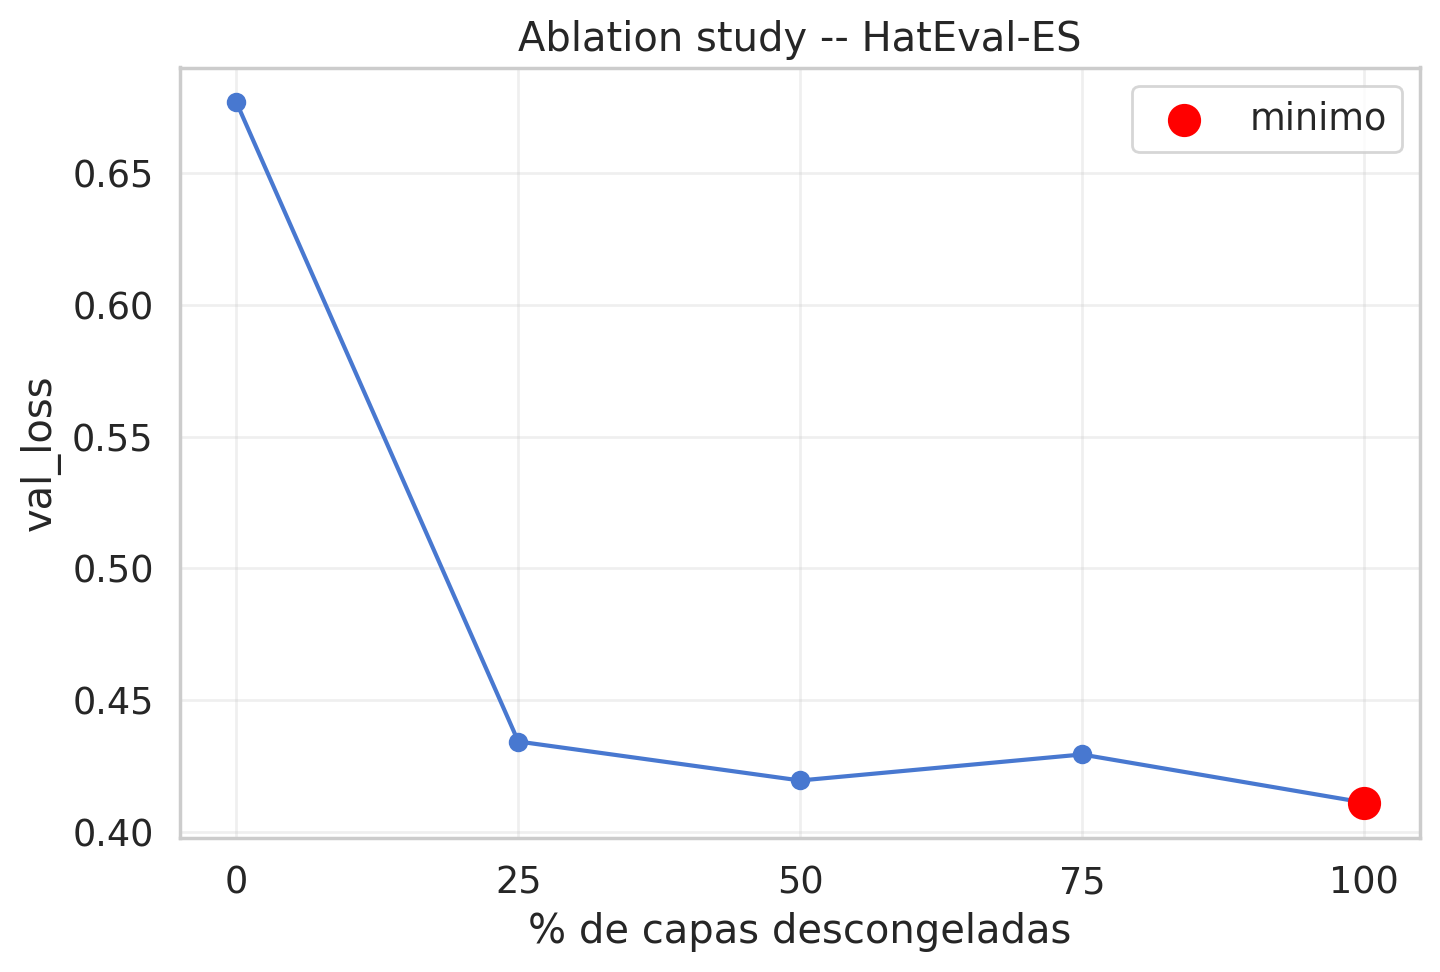
\includegraphics[width=0.85\linewidth]{fig_ablation_curve_s43.png}
\caption{\textit{Val\_loss} en función del porcentaje de capas descongeladas (semilla 43).}
\label{fig:ablation}
\end{figure}

La Figura~\ref{fig:trainval} muestra la evolución de \textit{train\_loss} y \textit{val\_loss} por época para esta configuración ganadora: el mínimo de \textit{val\_loss} (0.411) ocurre en la época 2, mientras que \textit{train\_loss} continúa descendiendo hasta valores cercanos a 0 en las épocas siguientes —evidencia directa de sobreajuste progresivo que \texttt{EarlyStopping} (\textit{patience}=2) detiene dos épocas después del mínimo, preservando el \textit{checkpoint} de la época 2 en lugar del de la época final.

\begin{figure}[h]
\centering
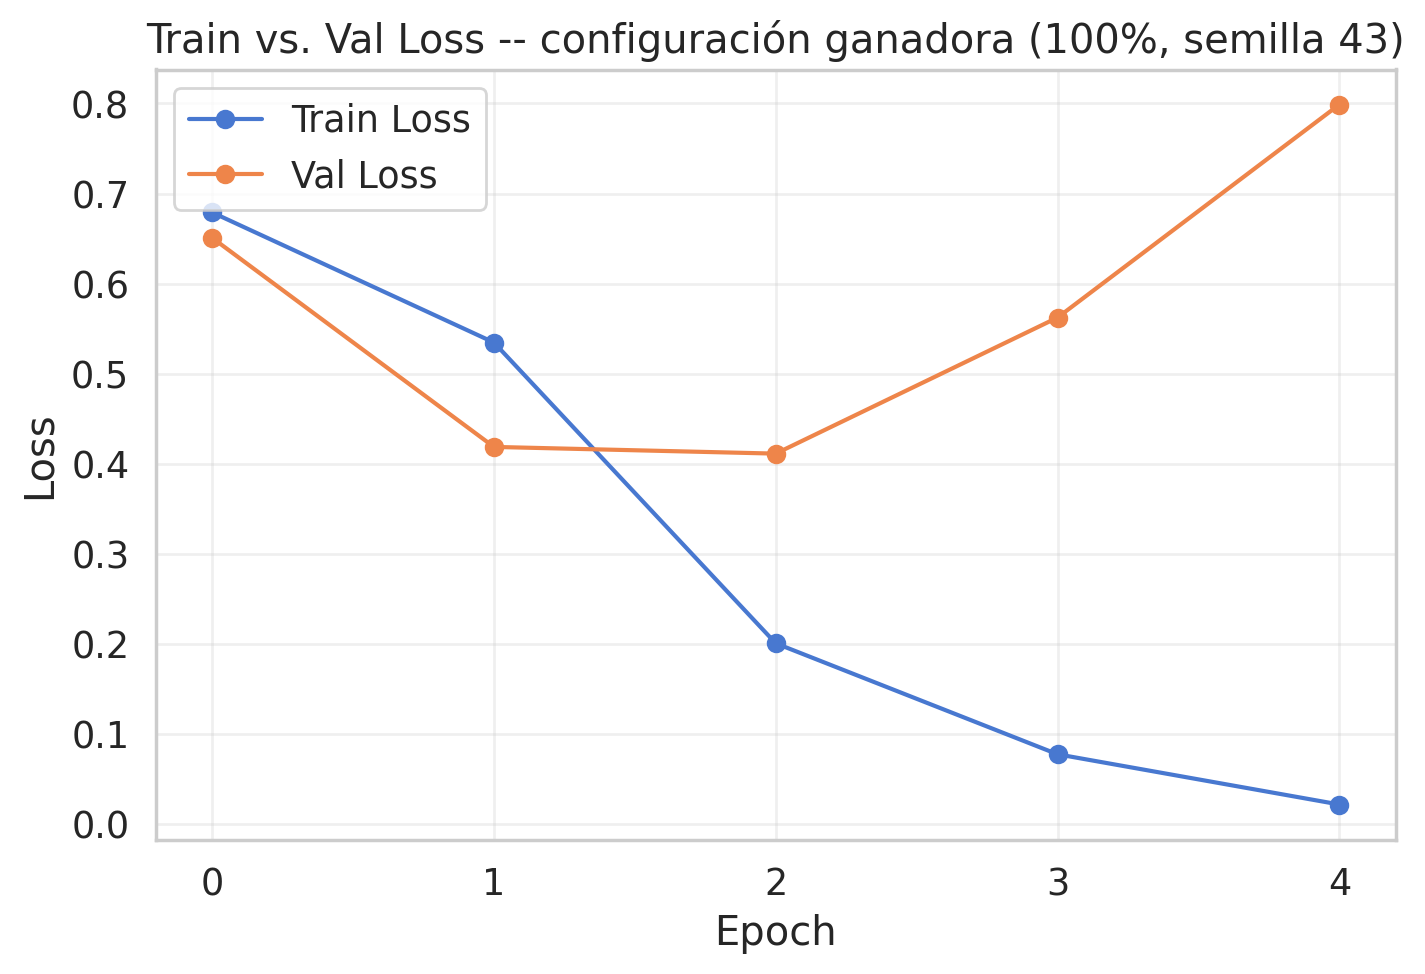
\includegraphics[width=0.95\linewidth]{fig_train_val_curve_s43.png}
\caption{\textit{Train\_loss} y \textit{val\_loss} por época, configuración ganadora (100\% descongelado, semilla 43).}
\label{fig:trainval}
\end{figure}

\textbf{Interpretación del patrón 0\% vs. 25--100\%.} La brecha entre 0\% y el resto no es gradual sino un salto: con el \textit{encoder} completamente congelado, la única adaptación posible es una transformación lineal sobre un embedding no orientado a la tarea, una limitación estructuralmente equivalente a la observada con Regresión Logística sobre BETO puro en la Sección~\ref{sec:cv-comparison} (F1=0.684) —ambas configuraciones explotan, en esencia, la misma representación estática. La literatura sobre la estructura interna de BERT indica que sus capas superiores concentran información semántica de más alto nivel, mientras las capas inferiores capturan sintaxis y léxico genérico, más transferible entre tareas \cite{jawahar2019bert}. Descongelar el 25\% superior (3 de 12 capas) ya da acceso a la porción del \textit{encoder} más relevante para reorganizar el embedding hacia la tarea, capturando la mayor parte de la ganancia alcanzable; descongelar capas adicionales aporta beneficio marginal decreciente, con diferencias entre configuraciones dentro de ese rango que se examinan formalmente en la Sección~\ref{sec:robustez}. Esto indica que, para esta tarea, no es cierto que ``más descongelamiento sea siempre mejor'': existe un umbral de saturación relativamente bajo, más allá del cual el costo computacional adicional no se traduce en mejoras reales de desempeño.

\subsection{Comparación BETO puro vs. ajustado}
\label{sec:cv-comparison}
La Tabla~\ref{tab:cv} resume la validación cruzada. La mejora fue sistemática en las cuatro familias de clasificadores (entre +0.210 y +0.406 de F1), siendo más pronunciada en \textit{Random Forest} (+0.406): este clasificador, basado en particiones ortogonales del espacio, rindió notablemente peor que los demás sobre BETO puro (F1=0.537 frente a 0.640--0.735), pero alcanzó un desempeño casi equivalente al mejor clasificador tras el ajuste (F1=0.944 frente a 0.945 de SVM). Esto sugiere que el \textit{fine-tuning} no solo mejora la calidad general del embedding, sino que también lo hace más favorable para una gama más amplia de clasificadores posteriores, no únicamente para el de mejor desempeño individual.

\begin{table}[h]
\centering
\small
\begin{tabular}{lcc}
\toprule
\textbf{Clasificador} & \textbf{BETO puro (F1)} & \textbf{BETO ajustado (F1)} \\
\midrule
Reg. Logística & 0.684 & 0.919 \\
SVM (RBF)       & 0.735 & 0.945 \\
Random Forest    & 0.537 & 0.944 \\
Gradient Boosting & 0.640 & 0.943 \\
\bottomrule
\end{tabular}
\caption{F1 promedio de validación cruzada (CV) repetida (5$\times$5) sobre \texttt{train+val}, HatEval-ES, semilla 43.}
\label{tab:cv}
\end{table}

\subsection{Evaluación en conjunto de prueba y separabilidad}
La mejor combinación (embeddings ajustados + SVM) alcanzó \textit{accuracy}$=0.830$ sobre el conjunto de prueba ($n=990$; IC 95\%: {[}0.807, 0.854{]}), sin sesgo marcado hacia ninguna clase (Tabla~\ref{tab:report}). Este valor es inferior al F1 de validación cruzada reportado en la Tabla~\ref{tab:cv} (0.945) porque mide un conjunto distinto: la Tabla~\ref{tab:cv} evalúa sobre particiones de \texttt{train+val}, mientras que la Tabla~\ref{tab:report} evalúa sobre datos genuinamente no vistos por ninguna etapa del \textit{pipeline}. Esta brecha (0.945 a 0.830) es una brecha de generalización normal, no un indicio de sobreajuste severo: el resultado de prueba se mantiene muy por encima de la línea base de predecir siempre la clase mayoritaria (0.585), confirmando que la mejora observada en validación cruzada se sostiene, en su mayor parte, en datos genuinamente no vistos.

\begin{table}[h]
\centering
\small
\begin{tabular}{lcccc}
\toprule
\textbf{Clase} & \textbf{Precision} & \textbf{Recall} & \textbf{F1} & \textbf{Soporte} \\
\midrule
No odio & 0.86 & 0.85 & 0.85 & 579 \\
Odio    & 0.79 & 0.81 & 0.80 & 411 \\
\midrule
Macro avg & 0.82 & 0.83 & 0.83 & 990 \\
\bottomrule
\end{tabular}
\caption{Reporte de clasificación en el conjunto de \textbf{prueba} (\textit{test}, datos no vistos), semilla 43.}
\label{tab:report}
\end{table}

El \textit{silhouette score} sobre la proyección t-SNE del conjunto de prueba pasó de 0.025 (BETO puro) a 0.294 (BETO ajustado). Visualmente (Figura~\ref{fig:tsne}), la proyección de BETO puro (panel superior) muestra las clases completamente entremezcladas, mientras que la del BETO ajustado (panel inferior) exhibe regiones claramente dominadas por cada clase, aunque sin separación perfecta —consistente con un \textit{silhouette} moderado y no cercano a 1. Este resultado, obtenido mediante una métrica geométrica independiente de cualquier clasificador supervisado, corrobora que el \textit{fine-tuning} reorganiza el espacio de representación hacia el constructo objetivo, y no únicamente que un clasificador posterior aprende a explotar mejor un embedding que en el fondo permanece igual de mezclado.

\textbf{Comparación con el estado del arte de 2019.} El mejor resultado reportado en el \textit{subtask} A para español del \textit{shared task} original \cite{basile2019hateval} fue F1 macro=0.730 (alcanzado de forma empatada por los equipos mineriaUNAM, Atalaya y MITRE, de 35 sistemas válidos presentados). La Tabla~\ref{tab:sota} compara estos resultados contra el desempeño de \textbf{prueba} (no de validación cruzada) del modelo de este trabajo.

\begin{table}[h]
\centering
\small
\begin{tabular}{lc}
\toprule
\textbf{Sistema} & \textbf{F1 macro} \\
\midrule
mineriaUNAM (2019) & 0.730 \\
Atalaya (2019) & 0.730 \\
MITRE (2019) & 0.730 \\
\textbf{Este trabajo (BETO ajustado + SVM)} & \textbf{0.830} \\
\bottomrule
\end{tabular}
\caption{Comparación con los mejores sistemas del \textit{shared task} original (\textit{subtask} A español). El valor de este trabajo corresponde al F1 de \textbf{prueba} (\textit{test}), no de validación cruzada.}
\label{tab:sota}
\end{table}

El modelo de este trabajo supera ese máximo histórico en +0.10 puntos absolutos (+14\% relativo). Esta diferencia es consistente con la brecha tecnológica de seis años entre ambos trabajos: los sistemas de 2019 se basaban predominantemente en SVM, LSTM y CNN sobre embeddings estáticos (GloVe, FastText); BERT, publicado apenas meses antes del \textit{shared task}, aún no había sido adoptado ampliamente por los participantes. El \textit{fine-tuning} de un \textit{transformer} contextual como BETO —inexistente como práctica estándar en ese momento— explica gran parte de esta mejora.

\begin{figure}[h]
\centering
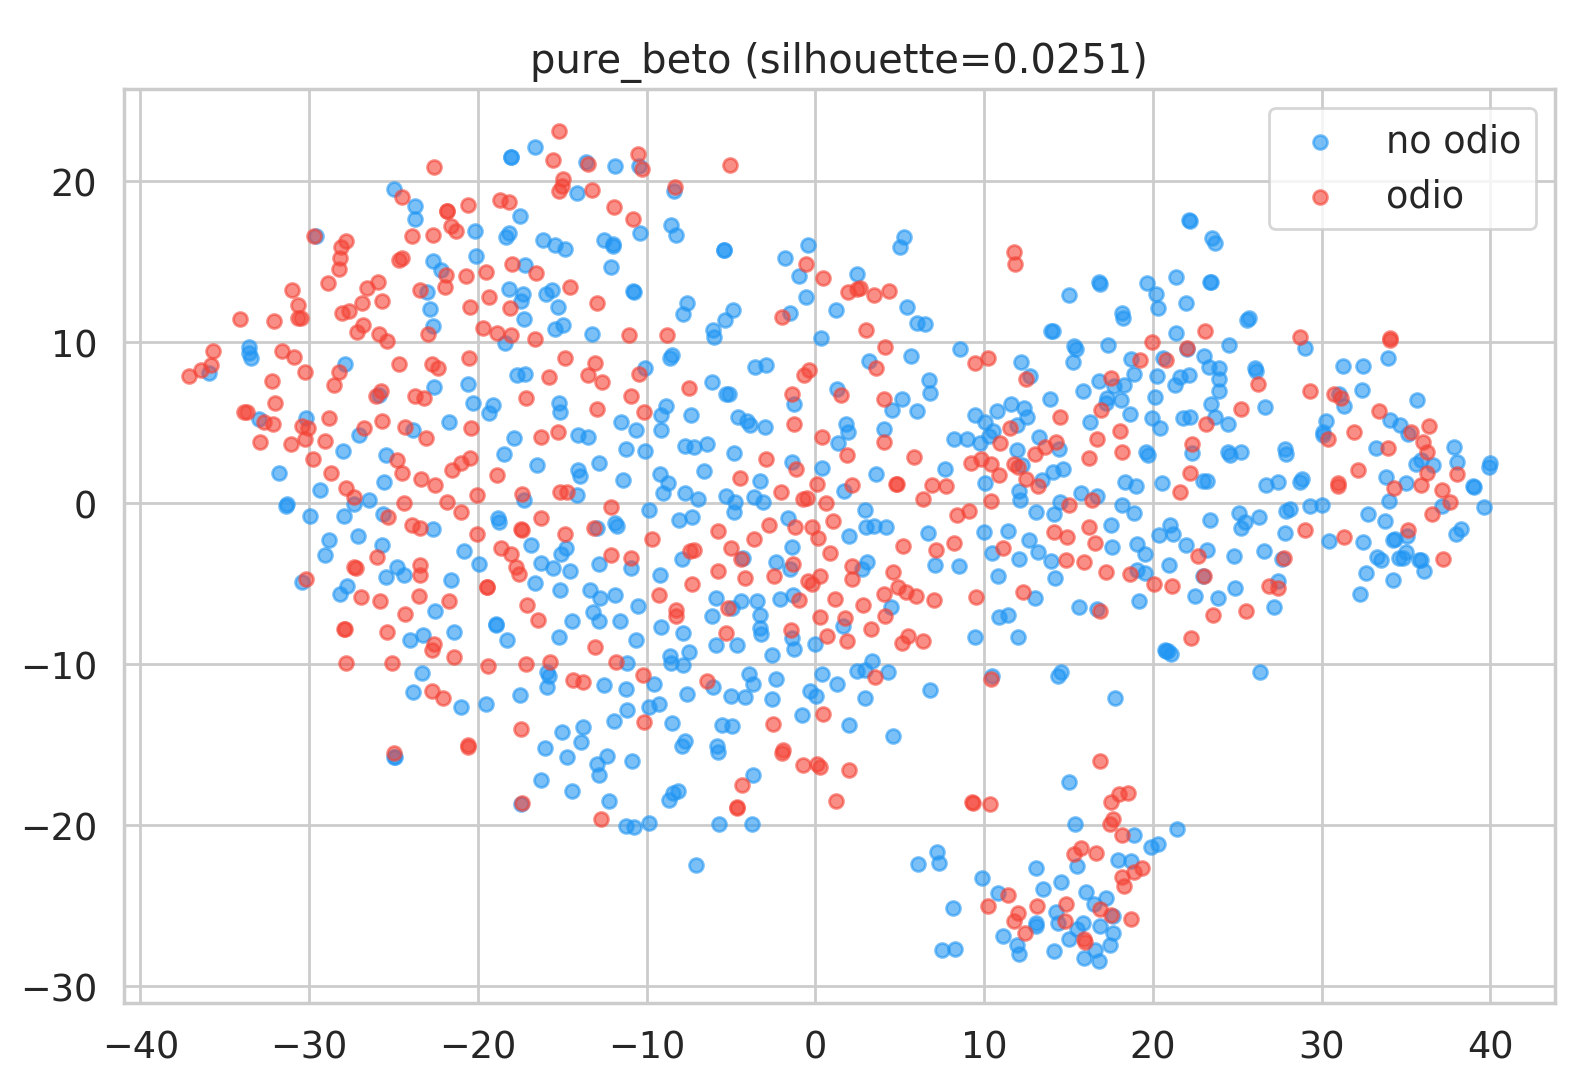
\includegraphics[width=0.95\linewidth]{fig_tsne_pure_s43.png}\\[2pt]
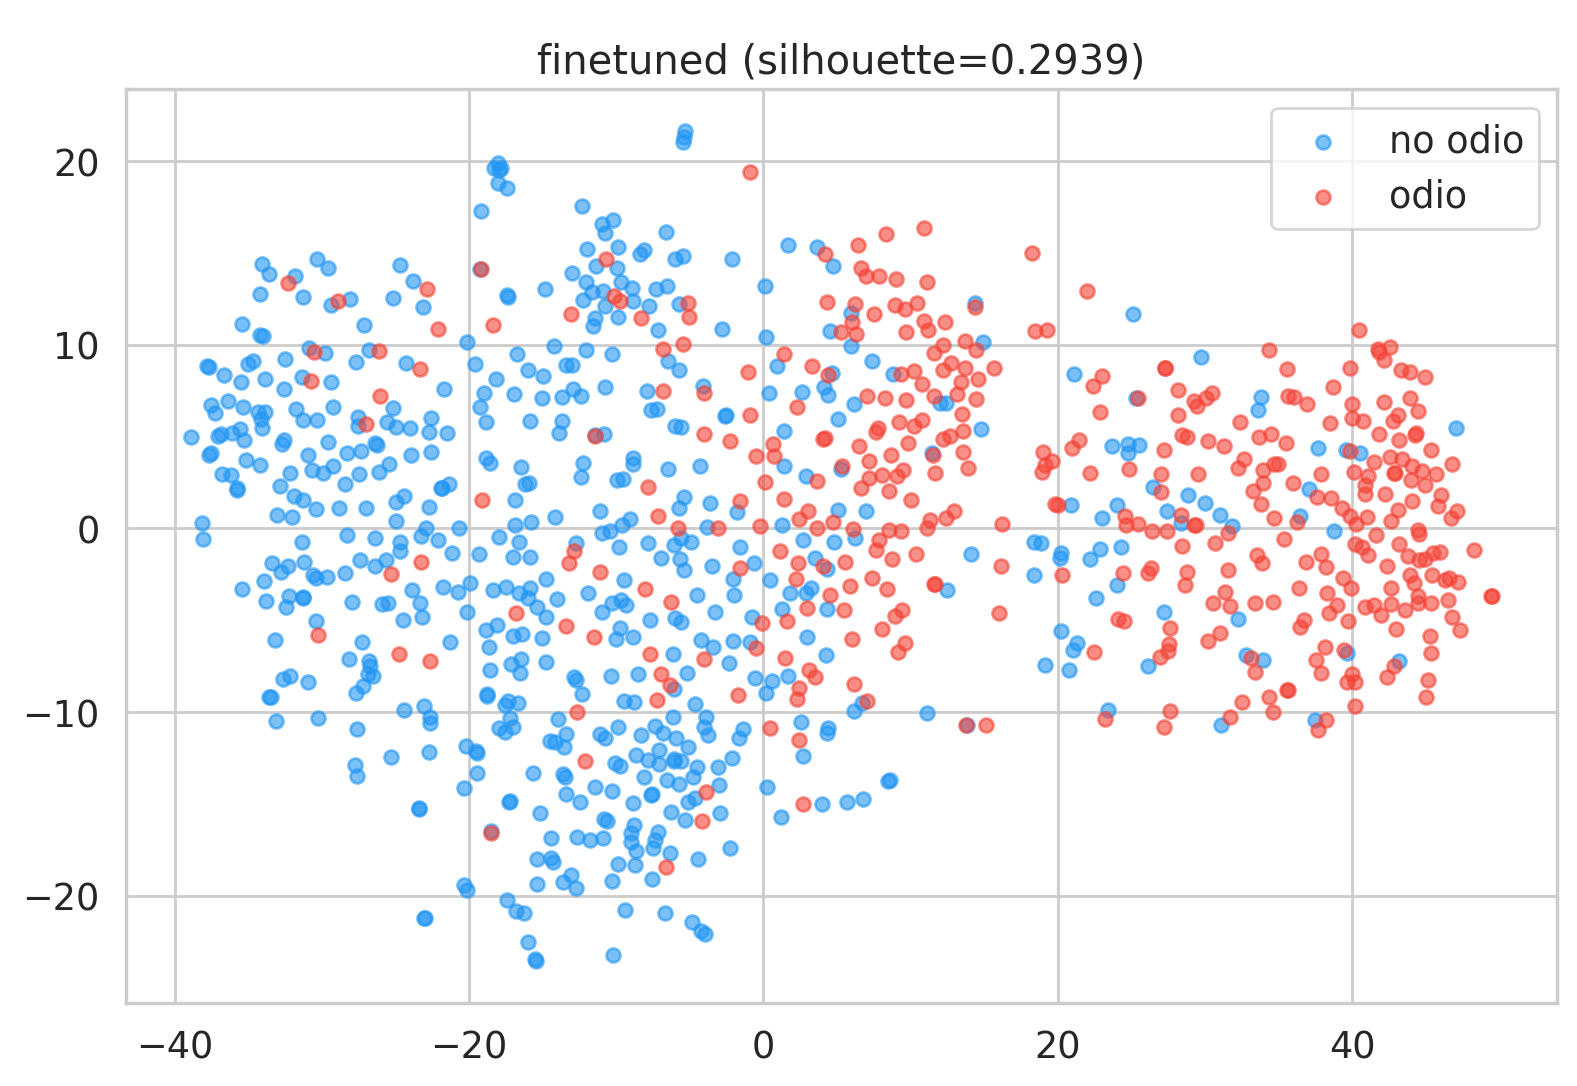
\includegraphics[width=0.95\linewidth]{fig_tsne_finetuned_s43.png}
\caption{Proyección t-SNE del conjunto de prueba: BETO puro (arriba) vs. BETO ajustado (abajo), semilla 43.}
\label{fig:tsne}
\end{figure}

\subsection{Verificación de robustez frente a la semilla aleatoria}
\label{sec:robustez}
Dado que la configuración óptima del \textit{ablation} podría depender de la inicialización aleatoria, se repitió el estudio completo con una semilla distinta (44, frente a 43 en el experimento principal), que además determina la partición entrenamiento/validación/prueba. La Tabla~\ref{tab:seed-comparison} compara el \textit{val\_loss} de ambas semillas para las cinco configuraciones.

\begin{table}[h]
\centering
\small
\begin{tabular}{lccc}
\toprule
\textbf{\% descongelado} & \textbf{val\_loss (s.43)} & \textbf{val\_loss (s.44)} & \textbf{$|\Delta|$} \\
\midrule
0\%   & 0.677 & 0.676 & 0.001 \\
25\%  & 0.434 & 0.398 & 0.036 \\
50\%  & 0.419 & 0.409 & 0.010 \\
75\%  & 0.429 & \textbf{0.383} & 0.046 \\
100\% & \textbf{0.411} & 0.404 & 0.007 \\
\bottomrule
\end{tabular}
\caption{Comparación de \textit{val\_loss} entre semillas 43 y 44. En negrita, la configuración ganadora de cada semilla.}
\label{tab:seed-comparison}
\end{table}

La configuración ganadora cambió de 100\% (semilla 43) a 75\% (semilla 44), con valores de \textit{val\_loss} para las cuatro configuraciones descongeladas contenidos en un rango de apenas 0.02--0.03 dentro de cada semilla —confirmando que la configuración óptima puntual del \textit{ablation} no es estable entre ejecuciones, y que el nivel exacto de congelamiento (superado el umbral de 25\%) no debe interpretarse como una elección crítica.

Pese a esta inestabilidad en el nivel de detalle del \textit{ablation}, el resultado central del trabajo se mantuvo robusto: el \textit{accuracy} de prueba fue de 0.842 (IC 95\%: {[}0.820, 0.865{]}) bajo la semilla 44, frente a 0.830 bajo la semilla 43 —intervalos de confianza que se solapan casi por completo— y el \textit{silhouette score} del embedding ajustado fue de 0.298 frente a 0.294, ambos muy por encima del BETO puro bajo la misma semilla (0.027 y 0.025, respectivamente). Esto indica que, si bien la configuración de congelamiento óptima es sensible a la inicialización aleatoria, la magnitud y consistencia de la mejora del \textit{fine-tuning} frente a BETO sin ajustar no lo son.

\section{Conclusiones}

Este trabajo muestra que el \textit{fine-tuning} supervisado de BETO mediante \textit{mean pooling} y una cabeza de clasificación lineal reorganiza su espacio de embeddings de forma sistemática y verificable para la tarea de detección de discurso de odio en español: la mejora se observa de manera consistente en cuatro familias distintas de clasificadores clásicos, se sostiene en un conjunto de prueba independiente muy por encima de la línea base trivial, y se corrobora mediante una métrica de separabilidad geométrica no supervisada (\textit{silhouette score}). El \textit{ablation study} de congelamiento de capas indica además que, superado el umbral de descongelar al menos una fracción moderada del \textit{encoder} (25\% o más), el nivel exacto de congelamiento tiene un efecto marginal sobre la calidad final del embedding, con diferencias entre configuraciones dentro del margen de variabilidad esperable de una sola ejecución.

\textbf{Limitaciones.} El \textit{dataset} fue recolectado en 2018--2019; el lenguaje de odio en redes sociales evoluciona, por lo que el desempeño reportado podría no generalizar a contenido actual. El alcance se limita a dos objetivos de odio (mujeres e inmigrantes), sin evaluar generalización a otras formas de discurso de odio. Como se muestra en la Sección~\ref{sec:robustez}, la configuración óptima exacta del \textit{ablation} de congelamiento no es estable entre semillas aleatorias, por lo que no debe interpretarse como una recomendación prescriptiva de un porcentaje específico, sino como evidencia de que descongelar al menos una fracción moderada del modelo es suficiente.

\textbf{Trabajo futuro.} Incorporar las subtareas \texttt{TR} y \texttt{AG} sobre el subconjunto de tuits ya identificados como odiosos; y evaluar el modelo ajustado sobre datos más recientes para estimar su vigencia temporal.

\begin{thebibliography}{9}
\small
\setlength{\itemsep}{0pt}
\bibitem{devlin2019bert} J. Devlin, M.-W. Chang, K. Lee, K. Toutanova, ``BERT: Pre-training of Deep Bidirectional Transformers for Language Understanding,'' \textit{Proc. NAACL-HLT}, 2019.
\bibitem{canete2020beto} J. Cañete, G. Chaperon, R. Fuentes, J.-H. Ho, H. Kang, J. Pérez, ``Spanish Pre-Trained BERT Model and Evaluation Data,'' \textit{PML4DC at ICLR}, 2020.
\bibitem{reimers2019sentencebert} N. Reimers, I. Gurevych, ``Sentence-BERT: Sentence Embeddings using Siamese BERT-Networks,'' \textit{Proc. EMNLP-IJCNLP}, 2019.
\bibitem{basile2019hateval} V. Basile, C. Bosco, E. Fersini, D. Nozza, V. Patti, F. M. Rangel Pardo, P. Rosso, M. Sanguinetti, ``SemEval-2019 Task 5: Multilingual Detection of Hate Speech Against Immigrants and Women in Twitter,'' \textit{Proc. SemEval-2019}, 2019.
\bibitem{jawahar2019bert} G. Jawahar, B. Sagot, D. Seddah, ``What Does BERT Learn about the Structure of Language?,'' \textit{Proc. ACL}, 2019.
\end{thebibliography}

\end{document}
